% --------------------------------------------------------------------
% This is a simple Beamer document that uses beamerthemesigpwny.sty
% Reading the comments should help you create a presentation even if
% you've never used Beamer before.
% --------------------------------------------------------------------
% Set our document class to Beamer
\documentclass{beamer}

% Some packages for nice font encodings in the final PDF
\usepackage[utf8]{inputenc}
\usepackage[T1]{fontenc}

% To insert images
\usepackage{graphicx}

% Useful packages from the AMS
\usepackage{amsmath,amssymb,amsthm}

% Package for code highlighting
\usepackage{minted}
\usemintedstyle{monokai}
\setminted{linenos=true, breaklines=true, breakanywhere=true, style=default}

% Set a title
\title{A Sample \TeX\ SIGPwny Presentation}

% The subtitle is generally where I'd expect you to put the week
% number, thus:
\subtitle{Week $\infty$}

% Whoever worked on the presentation:
\author{Pwny, Sig}

% A date, if you'd like.
\date{}

% An institute name, if you're so inclined
% \institute{University of Illinois Urbana-Champaign}

% Use the SIGPwny theme for this Beamer presentation
\usetheme{sigpwny}
% --------------------------------------------------------------------
% Begin document
\begin{document}

% Beamer calls each slide a "frame", defined within the environment:
% \begin{frame}
%   <frame content here>
% \end{frame}

% This frame is just the title.
\begin{frame}
\titlepage
\end{frame}

% A frame with the table of contents.
% This frame's title is "Outline".
\begin{frame}{Outline}
  \tableofcontents
\end{frame}

% The frame title is a flag.
\begin{frame}{sigpwny\{this\_is\_a\_flag\}}
  % Let's put some real content in this frame:
  Weekly updates:
  \begin{itemize}
    \item SIGPwny is an excellent cybersecurity club.
    \item I'm out of ideas for updates.
  \end{itemize}
\end{frame}

% Start a section: *sections* (subsections, etc.) are what show up in the TOC.
\section{Basics}
% Section pages can be printed thus:
\frame{\sectionpage}
% There's a way to automate this, see:
% https://tex.stackexchange.com/questions/178800/creating-sections-each-with-title-pages-in-beamers-slides/178803

% Another frame:
\begin{frame}
  % Alternate syntax for frame titles
  \frametitle{There Is No Largest Prime Number}
  % Frames can have subtitles:
  \framesubtitle{The proof uses \textit{reductio ad absurdum}.}
  % Some frame content:
  \begin{theorem}
    There is no largest prime number.
  \end{theorem}
  \begin{enumerate}
    % We do some interesting stuff with the items to make them appear
    % on sequential slides. See the PDF for how this turns out. The
    % first item is set to alert on the first slide in red.
    \item<1-| alert@1> Suppose $p$ were the largest prime number.
    \item<2-> Let $q$ be the product of the first $p$ primes.
    \item<3-> Then $q+1$ is not divisible by any of them.
    \item<4-> But $q + 1$ is greater than $1$, thus divisible by some prime
    number not in the first $p$ numbers.
    \item<5-> There exists a prime larger than $p$.
  \end{enumerate}
\end{frame}


\section{RSA}
\frame{\sectionpage}

% Similar for subsections:
\subsection{Some Intuition}
% And their pages:
\frame{\subsectionpage}

\begin{frame}
  \frametitle{Image}
  % This is how you'd include an image, centered.
  \begin{center}
    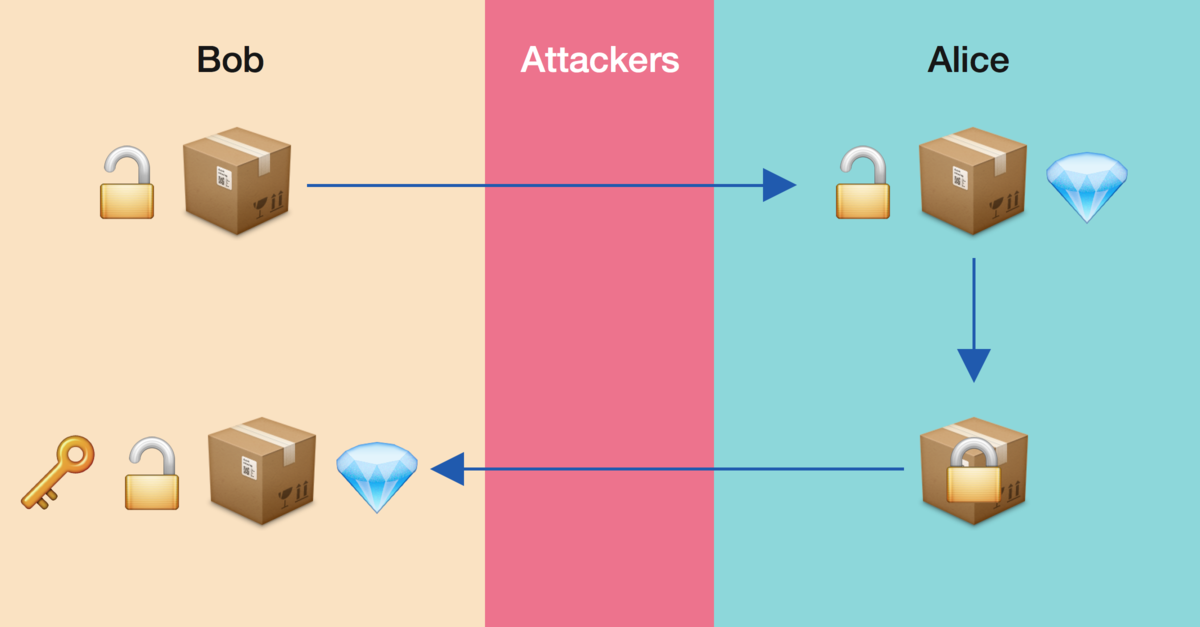
\includegraphics[width=0.8\textwidth]{rsa.png}
  \end{center}
\end{frame}

\subsection{The Math}
\frame{\subsectionpage}

\begin{frame}
  \frametitle{Key Generation}

  \begin{enumerate}
    \item Find primes $p$, $q$. Compute $n=pq$.
    \item Compute $\phi = (p-1)(q-1)$.
    \item Let $e$ be a number coprime to $n$.
    \item Compute $d = e^{-1} \pmod{\phi}$.
    \item $(n,e)$ is the \textbf{public key} tuple, $d$ is the \textbf{private key}.
  \end{enumerate}

\end{frame}

\begin{frame}
  \frametitle{Message Exchange}

  \begin{enumerate}
    % Note that we can use the SIGPwny colors the template makes
    % available to us anywhere we'd like:
    \item To send message $m$ to Alice, Bob computes $c = m^e \pmod{n}$
      using {\color{sigpwny@alertred} Alice's public key} $(n,e)$ and sends $c$ to Alice.
    \item Alice computes $m = c^d \pmod{n}$ to recover $m$.
  \end{enumerate}
\end{frame}

\begin{frame}
  \frametitle{Some Math Mode Testing}
  % Some fun with LaTeX Math
  $$\frac{x^2+3}{y^2+7}$$

  \[
    \mathcal L_{\mathcal T}(\vec{\lambda})
    = \sum_{(\mathbf{x},\mathbf{s})\in \mathcal T}
       \log P(\mathbf{s}\mid\mathbf{x}) - \sum_{i=1}^m
       \frac{\lambda_i^2}{2\sigma^2}
  \]

  $$\int_o^8 f(x) dx$$
\end{frame}

\begin{frame}[fragile]
  \frametitle{Some Sample Code}

  \begin{minted}{python}
    x = 10
    y = "mystring"
    print("Hello world!")
  \end{minted}

\end{frame}


\section{Conclusion}
\frame{\sectionpage}

\begin{frame}
  \begin{center}
    {\color{sigpwny@maingreen} So long, and thanks for all the fish!}
  \end{center}
\end{frame}

\end{document}